%%% 関西大学 総合情報学部 松下ゼミ 進捗報告 TeXテンプレート Ver 1.1 (2011/12/04) %%%
\documentclass{matsushita-zemi}
\usepackage[dvipdfmx]{graphicx}
\usepackage{comment}
\usepackage{ascmac}
\graphicspath{{./fig/}}

%%% タイトル (長くなる場合は¥¥で適宜改行すること)%%%
\title{Elucignage:ユーザの興味や関心への効率的なアクセスを可能にする可視化インタフェース}

%%% 氏名 (姓・名の間は半角スペース) %%%
\author{内藤 峻}

\begin{document}
\maketitle

%%% 以下、本文 %%%
\section*{概要}
\label{abstract}
ネットワーク上には多様な種類の情報が存在しており、それらをユーザの要求に応じて適応的にまとめ上げる技術が渇望されている。その一つとして、テキストなどの言語情報と統計データなどの数値情報の相補的な利用に関する研究が行われている。その一環として、本研究では言語情報と数値情報が密接な関係にある株価などの動向情報に着目しそれらを統一的な枠組みで可視化する手法を提案する。株価などの統計情報の場合、その正確な値を知るには数値情報が適切であるのに対して、変動の大局的な理解や背景となる事象の把握には言語情報が適している。そこで、これらを一つのグラフ上に提示し、その情報源に対話的にアクセスできるようにする。

\section{はじめに}
\label{background}
%電子化が普及している話
%それらの情報を利用して意思決定や問題解決に役立てられている話
%しかし、情報は膨大になっている、時間にともなって更に増加を続けている話
%既存の検索技術ではユーザの要求に答えることができない
%それらをまとめる技術が求められている話
%しかし、情報には様々な種類がある話
%本提案では数値情報(統計データ)と言語情報(新聞記事)に着目した話
近年、様々な情報が電子化されネットワーク上に蓄積されている。それに伴い、これらの情報を利用して意思決定や問題解決に役立てる試みがなされている。しかし、蓄積された情報は膨大であるうえ、時間の経過に伴って更に増加を続けている。そのため、"情報の在処を見つける"ことを主眼とした検索技術ではユーザの要求に十分に応えることができず、ユーザの関心や興味に合致する情報に直感的かつ簡便にアクセスするための技術、言うなれば"情報の理解   "を助ける技術が渇望されている\cite{Elucignage}。
このような要求に答える技術のひとつとして、本提案では統計データ等の数値情報と新聞記事等の言語情報を相補的に用いて編纂し、ユーザの情報アクセス行為を容易にする技術の実現をめざす\cite{information_compilation}。

ネットワーク上にはテキストや統計データ、音声、画像動画など様々な種類の情報が存在している。将来的にはそれらの情報全てを対象とし、状況や目的に応じて取捨選択やモード変換を行い、適切な形態で組み合わせてユーザに提供することが望まれるが、現在の技術レベルではその実現は容易ではない。そこで本研究では、まず時間的変動を伴う統計データ(時系列数値情報)とそれに関連する記事(言語情報)を対象とし、ユーザがそれらの情報にアクセスしたり、その概要を把握したりする際の支援となる可視化手法について議論する\cite{Elucignage-jsai}。

本稿では、まず、先行研究について述べる。次に、デザイン指針を説明し、その後、先行研究を示す。

\section{先行研究}
\label{relatedworks} 
動向情報を可視化する枠組みとして、山本らの可視化システム\cite{Tagged_corpus}や松下らのSTEND\cite{STEND}、加藤らのElucignage\cite{InformationcompiledStudyGroup}、高間らの地震情報可視化システム\cite{SpaceTrendInformation}などがある。

山本らは、動向情報の変化要因に関する重要語を注釈としてグラフに表示する方法を提案している(図\ref{system})\cite{タグ付きコーパス}。要因の抽出では、動向情報が記載された新聞記事と文章の類似度が高い新聞記事を要因としている。また、要因とされた新聞記事からのキーワード抽出は、1月分の新聞記事を1ドキュメントとみなしたTF・IDF値に基づき行っている。動向情報とその要因の表示方法に関するアンケート調査からは、ユーザが動向情報に関する要因を知りたいことは、動向情報を示したグラフ中の変化が大きい部分とその前後、最大位置と最小位置、及び最初と最後の3つに分類できることが分かったと述べられている。また、要因の表示方法としては、1ウィンドウに3つ程度のトピックを簡潔に示したものや、要因をタイトルやキーワードとともに表示すれば良いことが分かったと述べられている。

%山本らは、記事中に存在するある時点の変化についての定性的な記述や、原因や影響に関する記述を注釈としてグラフに与える方法を提案している\cite{Tagged_corpus}。例えば内閣支持率の場合、過去のある時点の支持率と関係が強い出来事を注釈することで、どのような事件が支持率に影響を与えたかをユーザが把握・判断できるようにしている。値の変化の大きな点、減少から増加に転じる極小点など、利用者が関心を持ちそうな点に選択的に情報を付与することによって視認性の向上を測り、ユーザにとって分かりやすい情報提示を目指している。

%この方法は本稿の提案方法と問題意識が近く、特に情報提示に関しては参考になる点も多い。しかし、その情報提示がユーザとのインタラクションにおいてどのように作用し適応していくかについては、現状ではあまり深く検討されていない。本提案はユーザのインタラクションに基づく適応的情報提示に大きな関心があり、この点でこれらの方法と方向性が異なる。
\begin{comment}
 \begin{figure}[tb]
   \begin{center}
    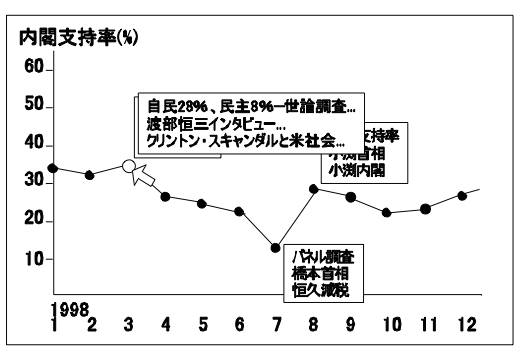
\includegraphics[width=8cm,bb=0 0 521 356]{tagu.PNG}
   \end{center}
  \caption{山本らのシステムの出力例}
  \label{system}
 \end{figure}
\end{comment}

松下らは、グラフ概形を示唆するシステムSTENDを提案している\cite{STEND}。STENDは時系列数値情報を扱わず、新聞記事のテキストデータのみから取得可能な数値情報と定性情報に着目してグラフ描画を試みたものであり、本提案とは力点が異なる(図\ref{STEND})。テキスト中の「昨年10月より約40%の下落になっている」「前年同月に比べて5ドル上昇した」等の比較表現や「安定傾向にあった」「10月をピークに下落している」等の定性表現から情報を抽出している。情報提示では、統計グラフを用いず数種類の点や短形、形状の異なる幾つかの矢印記号を組み合わせることでその代替を試みている。
\begin{figure}[tb]
  \begin{center}
   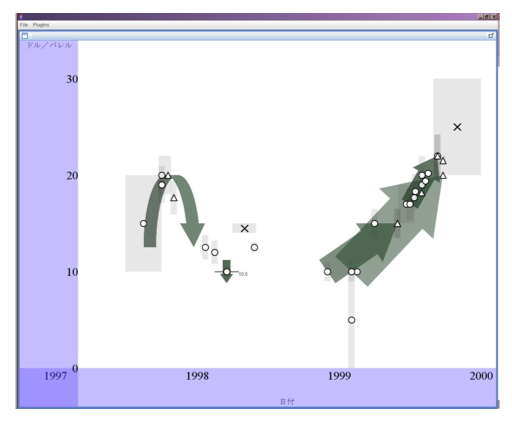
\includegraphics[width=8cm,bb=0 0 512 422]{STEND.PNG}
  \end{center}
 \caption{STENDの描画例}
 \label{STEND}
\end{figure}
加藤らは、グラフに文章を関連付けた視覚オブジェクトを提案している\cite{InformationcompiledStudyGroup}。2つの画面を上下に配置しており、上画面にグラフ概形(図\ref{oblject}上画面)、下画面に状況記述を表現している(同下画面)。また、下画面ではグラフ上のアイコンに対応する記事の一部が表示されている。この記事とグラフは一方を選択すると他方の対応する部分がハイライトする等の対応付けがなされている。
さらに、視覚オブジェクトの操作として、グラフ表示を操作するためのパネルがグラフの右下に配置されている。これを使って、表示する期間の変更や、拡大縮小が行える。そのため、これらの視覚オブジェクトを介して特徴点や文書の閲覧が行われる必要があるとされている。これら全般を扱うインタラクションの設計が必要となると述べられている。
\begin{comment}
 \begin{figure}[tb]
   \begin{center}
    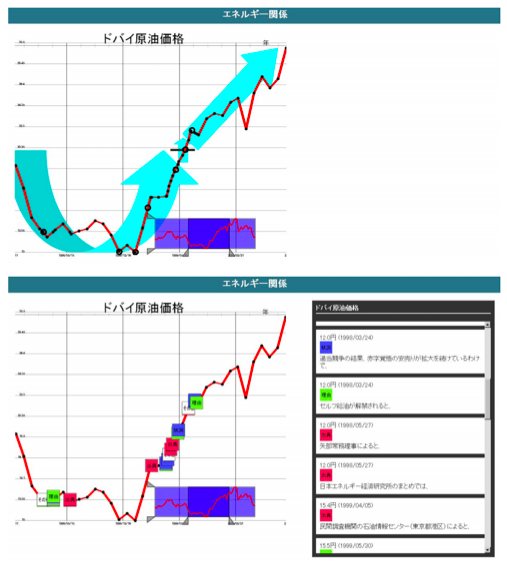
\includegraphics[width=8cm,bb=0 0 507 566]{object.PNG}
   \end{center}
  \caption{文章とグラフを関連付けた視覚オブジェクト}
  \label{oblject}
 \end{figure}
\end{comment}

小泉らは言語情報と統計グラフとを意味のレベルで処理するために、被験者実験を通じて実際に使われる語彙の分析と文書構造の解析を行っている\cite{interconversion}。
グラフをどのように言語として表現しているのか分類している。グラフを左から右だと「左右」、全体だと「全体」、左右の後に全体を示している場合は「左右+全体」など計5つの分類を行っている。
その結果、文章の構造を語彙の出現頻度によっておおよそ分類可能であることを示している。
これは本研究のElucignageの矢印アイコンの選定に有効であると考える。

%%%少なすぎる%%%
高間らは動向情報だけでなく空間的な動向情報を含んだ可視化システムついて提案している\cite{SpaceTrendInformation}。
地震や台風などは時間的な動向情報だけでなく空間的な動向情報を含んでおり、両者を考慮した可視化が必要となる。
地図とグラフ、それに対応する新聞記事を一画面に提示している。
複数の地震について同じ空間へ描画することを可能にしている。
本システムの展望として、動向情報だけでなく、空間情報もシステムの機能として付与したい。

太田らは文書中の数値的特徴を用いた情報可視化につて述べている\cite{numerical_features}。
この論文では、記事から抽出されたデータの特徴を基に適切なグラフの種類を決定し、グラフの作成を行う手法について述べている。折れ線グラフは時間経過による数量の変化を視覚的に表示するときにてきしていることや、棒グラフは数量の比較を視覚的に表示するときに適しているなど、各グラフの特徴について詳しく述べられており、参考になった。

\section{デザイン指針}
%目的をどのように達成するのかという話
%どのような機能が必要なのか?何故必要なのか?
%シナリオに基づいた話
%必要な機能な整理
%シナリオを載っけるのもあり
%言語情報と数値情報を扱う話
%それらをどのように見せるか、どのようなインタラクションを想定するのかという話
%変化の実験の論文を引用
%統計情報等の数値情報は正確である。
%変わって、言語情報はあいまいであるものの、その時点の背景等を理解することができる。
%本研究では、数値情報には統計DBを、言語情報には新聞記事を用いて、ユーザの効率的なアクセスを促すシステムを提案する。
%ユーザの効率的なアクセスを支援するためにはユーザのふるまいを想定をする必要がある。
%ユーザはグラフを見て、そのときの変化における要因や背景を知りたいと思う。そこで、本提案ではユーザの興味や関心を想定したインタラクションを考える。
%ユーザはグラフの変曲点になる部分に興味を持つ。
%また、そこで、要因と背景を知りたいと思う。
%以下の様なシナリオを想定している。
本研究では提案システムをデザインするにあたってシナリオ手法を用いる。そして、必要な機能を整理する。以下にシナリオの例を示す。
\begin{screen}
工場を経営しているAさんは最近、自社で扱っているガソリンの価格が上昇していることを知り、不安に思い始めた。そこで、最近のガソリンの価格を調べることにした。すると、ガソリンの価格はある程度上下するものだとわかった。しかし、ある程度上下するものの価格は上昇傾向にあった。何故、上昇傾向にあるのか調べてみると、背景に外国情勢が絡んでいた。一つはウクライナ情勢である。産油国のロシアから欧州への原油供給が止まる可能性が取りざたされていた。さらに、同じく産油国のイラクでも6月から武装組織が活動を活発化させ、原油の供給が脅かされていることや円ドル相場が2013年初頭と比べ10\%ほど円安になり、輸入コストが増大していること、さらには、経営の厳しさが増す国内の石油元売各社やガソリンスタンドが、収支改善のために原料の上昇分を店頭価格に反映させ始めたとの指摘もあることがわかった。念のため、円ドル相場を調べてみると、2013年初頭と比べて円安になっていた。調べていくうちに、もしかすると「夏にガソリンの価格が上がるのではないか」と考え、過去の3年分のデータを調べることにした。すると、夏と冬をピークに価格が上下することがわかった。また、2008年に価格が急上昇しているのをみて、何故こうなったのか原因を調べることにした。調べてみると、アメリカの金融危機が原因だとわかった。Aさんは不安を解消することができ、安心してガソリンを購入しようと決意した。
\end{screen}



\section{今までやったこと}
\begin{comment}
\subsection{概要}
%書き直し、もう少し詳しく述べられるはず
ユーザは統計グラフの外観を理解するだけでなく、興味を持った箇所についてどのようなことが述べられているかをその要因となる記事にアクセスすることで参照できる。そのため、ユーザの関心がある動向情報を時系列数値情報を用いて統計グラフとして描画し、そのグラフの要因となる記事をその内容に適したアイコンの形式で提示する方法を採用する。このアイコンは要因となる記事のアクセスを可能にする。また、記事の一部を画面の一部に表示し、そこからグラフのどの部分に該当しているかを示す機能を備える。これにより、要因となる記事がグラフのどの部分で記述されたものであるかを確認できる。

\subsection{実装}
\end{comment}
%現段階の実装に関して述べる。
%検索ボックス
%記事リストパネル
%グラフパネル
%コントロールパネル
%使ったデータの図を貼る
試作したElucignageプロトタイプの外観を図\ref{Elucignage}に示す。システムはHTML、CSS、javascriptを用いて実装した。javascriptのライブラリはjquery-1.6.2.jsとD3.jsを用いている。現在はガワとグラフの描画、新聞記事を提示する機能を実装したところである。
このプロトタイプは、記事リストパネルに新聞記事を表示するボタン、記事のスニペット(snippet)を表示する記事リストパネル、グラフとそれに関連する記事へのポインタであるアイコンを表示するグラフパネルから構成される。
ユーザがボタンをクリックすると、記事リストパネルに記事の一覧がスニペットを伴って表示される。スニペットはユーザに元記事を参照する価値があるかどうかの判断材料として提示されるものである。グラフパネルにはシステム起動時にグラフとアイコンが表示される。
現在の実装はボタンがクリックされるかどうかを判定し、クリックされると新聞記事の一部を提示するようになっている。また、スニペットはxml形式のファイルからTEXTタグに含まれている本文を表示させている。グラフはD3.jsを用いて描画している。アイコンはクリックされると記事のスニペットの文字が大きくなる\ref{Elucignage_click}。これはユーザが興味や関心のある新聞記事へ誘導するためにフォーカスするためのものである。

\begin{figure}[tb]
  \begin{center}
   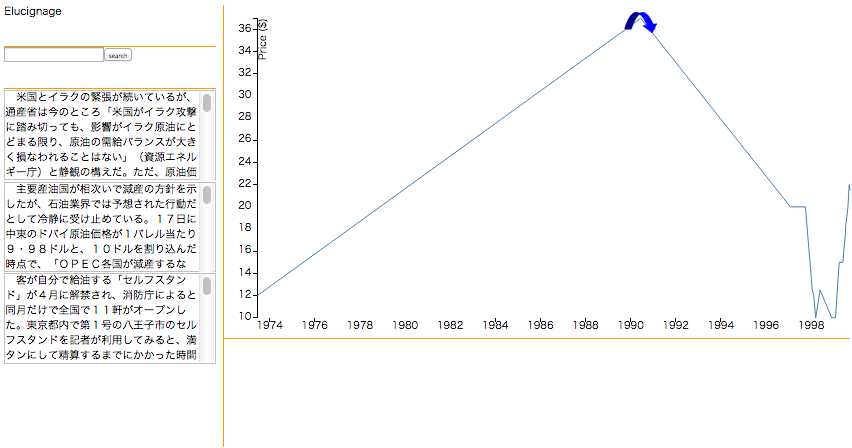
\includegraphics[width=8cm,bb=0 0 852 448]{Elucignageprototype.png}
  \end{center}
 \caption{Elucignageのスナップショット}
 \label{Elucignage}
\end{figure}
\begin{figure}[tb]
  \begin{center}
   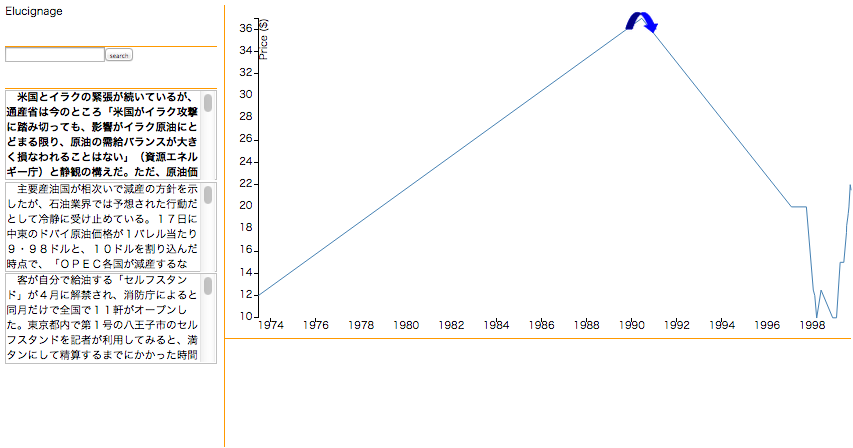
\includegraphics[width=8cm,bb=0 0 853 448]{Elucignage_click.png}
  \end{center}
 \caption{Elucignageのスナップショット(アイコンをクリックしたとき)}
 \label{Elucignage_click}
\end{figure}

\section{これからやること}
%ボタンを検索可能な検索ボックスにする
%スニペットには指示的な要約を用いる
%関連記事の同定や選択、スニペットの生成の自動化
%コントロールパネル(オーバービューエリアを含めた)を実装する
%アイコンの自動生成
この章ではこれから実装する予定である機能を示す。まず、グラフの描画範囲を変更することができるコントロールパネルを実装する。次に、検索を可能にする。ボタンを検索ボックスにし、統計情報の一部を入力すると、グラフパネルにグラフとアイコンが表示されるようにする。同時に、記事リストパネルに関連する記事の一覧がスニペットを伴って表示されるようにする。その後は、関連記事の同定や選択、スニペット、アイコンの生成の自動化を考えていく。


\section{おわりに}
本稿では、動向情報の可視化手法について考察した。先行研究として山本らの可視化システムや松下らのSTEND、蓮井らのグラフ型インタフェース、加藤らの視覚オブジェクトを報告した。続いて、卒業研究への展望を示した。

%%% 参考文献 %%%
\bibliographystyle{ipsjsort}
\bibliography{reference}

\end{document}